\section{Dados Pessoais}
Nesta seção iremos descrever propostas de melhorias para a aplicação de consulta pública utilizada no anteprojeto de lei de \pdp.

\subsection{Respostas a comentários}
	O primeiro ponto que demanda melhoria é a principal funcionalidade do aplicação – comentários nos trechos do ante-projeto de lei.
	Atualmente a plataforma apenas permite que os usuários opinem trechos do texto, conforme mostra a Figura \ref{fig:comentarios-dados-pessoais-hoje}.
    \begin{figure}[htb]%
        \begin{center}
            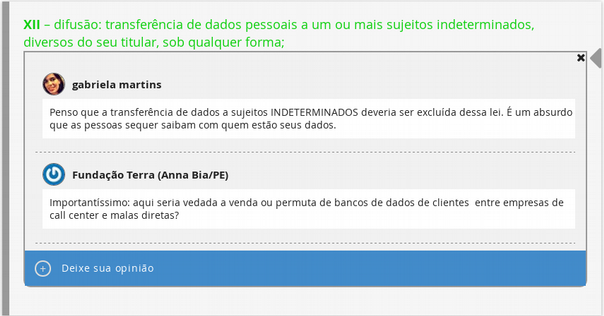
\includegraphics[scale=0.6]{./imagens/dados-pessoais-atual.png}%
        \end{center}%
        \caption{Situação atual dos comentários na ferramenta da consulta ``\pdp''\label{fig:comentarios-dados-pessoais-hoje}}%
        \fonte{Autoria Própria}%
    \end{figure}%
    
Como o objetivo é que haja um debate, é fundamental permitir que os usuários possam responder a comentários feitos, e que isso seja apresentado na forma de comentários agrupados e aninhados, permitindo um melhor desenvolvidomento do debate propriamente dito. Assim, propõe-se que seja implementado o recurso de resposta a comentários, conforme pode ser observado na Figura \ref{fig:comentarios-dados-pessoais-proposta}.
    \begin{figure}[htb]%
        \begin{center}
            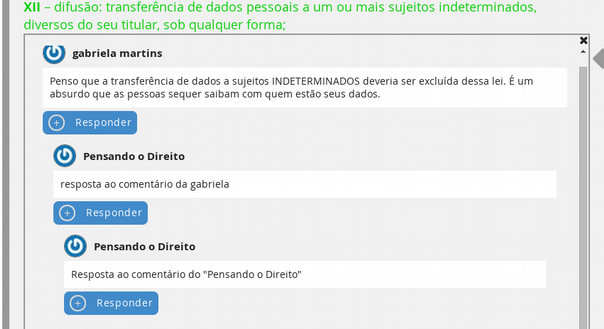
\includegraphics[scale=0.6]{./imagens/dados-pessoais-comment-novo.png}%
        \end{center}%
        \caption{Proposta de modificação com ``Respostas'' \label{fig:comentarios-dados-pessoais-proposta}}%
        \fonte{Autoria Própria}%
    \end{figure}%
    
\subsection{Implementação}
Para se chegar a tal resultado, será necessário modificar o plugin “wp-side-comments” e também realizar modificações no tema do wordpress utilizado na aplicação (“dadospessoais-tema”).
	Com relação ao plugin ``wp-side-comments'', a implementação passará por algumas modificações pequenas nos arquivos ``wp-side-comments.php'' e ``wp-side-comments.js'' e por grandes modificações no arquivo ``side-comments.js'', plugin javascript independente que implementa a funcionalidade de ``comentários laterais''.
	Relativo ao tema “dadospessoais-tema”, será necessário modificar o arquivo ``dadospessoais.js'' para implementar o template e alguma lógica para as respostas, além do desenvolvimento de regras de estilo CSS.
	
\subsection{Concordar / Discordar}
Outra possibilidade a ser ponderada é a adição de botões ``concordar'' e ``discordar'', permitindo que os usuários interajam com os comentários/respostas de outros usuários pode meio de endossos ou reprovações de opiniões já expressas.
	Deve-se ponderar a utilização deste recurso pois, por um lado, ele pode desestimular a participação dos usuários por meio da expressão escrita de suas opiniões, restringindo-se a ``votar''. Por outro lado, este seria um recurso de grande valia para a sistematização das contribuições feitas na consulta.
	Como forma de tentar estimular colaborações textuais, reduzindo o efeito negativo do recurso ``voto'', após o usuário votar poderia ser apresentado a ele um ``box'' convidando-o a expor os motivos pelos quais ele concorda ou discorda – a depender do voto dado; daquele comentário. Assim, uma ação simples e rápida (voto) pode vir a ser convertida num texto que complemente uma opinião anteriormente exposta ou num texto que exponha pontos de fragilidade de um argumento.
	Este recurso poderia ser desenvolvido enquanto uma \textit{feature} do plugin ``wp-side-comments'' de forma que esta feature possa ser ativada ou desativada, permitindo assim sua utilização quando for considerada conveniente.
	
\subsection{Redes Sociais}
Outro recurso que pode contribuir para o debate público, caso venha a ser implementado, é permitir que os usuários compartilhem trechos específicos do texto em debate nas redes sociais, ou que ao inserir um comentário na aplicação que este comentário seja automaticamente distribuído na rede social com o link de referência de volta para o comentário. Desta forma, pode-se potencializar o debate e atrair novas pessoas por meio da atuação dos próprios usuários.

\subsection{Implementação}
	A implementação deste novo recurso também passará por modificações no plugin ``wp-side-comments'' e no tema ``dadospessoais-tema''. Será preciso implementar um link permanente (permalink) para cada trecho de texto e/ou comentário, de forma que este permalink possa ser compartilhado nas redes sociais, dando acesso direto ao trecho ou comentário.